\documentclass[aspectratio=169]{beamer}
\usepackage{beamerthemetot}
\usepackage{graphicx}
\usepackage{animate}
\usepackage{calligra}
\usepackage[absolute,overlay]{textpos}
\usepackage[T1]{fontenc}
\usefonttheme{professionalfonts}
\usepackage{tikz}
\usetikzlibrary{shapes,arrows}
\usepackage{xcolor}
\usepackage{mathtools}
\usepackage{cancel}
 

\newcommand{\mytitle}{\color{White}\huge{\textbf{Data-Scarce Solid Mechanics Problems}}}
\newcommand{\mysubtitle}{\color{Pink}\Large{\textbf{New Machine Learning Strategies for Data Scarce Material Science Problems}}}
\newcommand{\myauthor}{\color{White}\textcalligra{\LARGE Ozgur Taylan Turan}}
\newcommand{\authorlabel}{\small O.T. Turan}
\author{\authorlabel}
\setbeamercovered{transparent}
\usepackage[backend=bibtex,firstinits=true,maxnames=30,maxcitenames=20,url=false,style=authoryear]{biblatex}

\setlength\bibitemsep{0.3cm} % space between entries in the reference list
\renewcommand{\bibfont}{\normalfont\scriptsize}
\renewcommand{\cite}[1]{\footnote<.->[frame]{\fullcite{#1}}}
\setbeamertemplate{bibliography item}{}
\bibliography{../../../Mendeley/bibtex_linux/GNG.bib}

\begin{document}

{
\def\beamer@entrycode{\vspace*{-\headheight}}
\setbeamertemplate{frametitle}[default][center]
\setbeamertemplate{navigation symbols}{}
\usebackgroundtemplate{
\includegraphics[width=\paperwidth,height=\paperheight]{cover/coverart.pdf}}

\begin{frame}[plain] 

\begin{minipage}{\textwidth}
	\centering{\mytitle} \\
	%\vspace{1cm}
	%\centering{\mysubtitle} \\
	\vspace{1cm}
	\centering{\color{White}November 15, 2021} \\
	\vspace{1cm}
	\centering{\myauthor}\\
\end{minipage}
\end{frame}
}


\begin{frame}
  \centering
  \mysubtitle
\end{frame}

\begin{frame}{Outline}
  \centering
  \begin{itemize}
    \item Introduction to Modeling
    \item Modeling Composites
    \item Machine Learning in Mechanics
    \item Observations \& Possible Paths
    \item Summary
  \end{itemize}
\end{frame}


% Meta Learning Definitions
%Learning to learn, also referred to as meta-learning, treats the training of a machine learning model as a learning problem in itself. In the context of this work if a machine learning model's performance on a task is improving with training experiences it is said to be learning. In the light of this definition a machine learning model is said to be learning to learn if the performance on each task improves with training experience obtained from each task and with the number of tasks \cite{thrun1998}. Meta-learning recently is being used to tackle few-shot learning problems, where there is little data available from the learning task that is of prime interest, whereas there is an abundance of data from other similar tasks. 

Learning to learn, also referred to as meta-learning, treats the training of a machine learning model as a learning problem in itself. In this setting, there exist multiple learning problems and the learning problems are treated altogether. Then, a machine learning model is said to be learning to learn if the performance on each task improves with training experience obtained from each task and with the number of tasks \cite{thrun1998}. Meta-learning recently is being used to tackle few-shot learning problems, where there is little data available from the learning task that is of prime interest, whereas there is an abundance of data from other similar tasks. 

% What Makes MAML Different
%Early works of the learning-to-learn paradigm relied upon the one supervisory and one sub-ordinate model that interacts with each other for meta-learning. On one hand, sub-ordinate models try to improve the performance with training examples and on the other hand, the supervisory model tries to increase the performance over the family of tasks. MAML (Model-Agnostic Meta-Learning) \cite{finn2017} is a model that circumvents the need for supervisory and subordinate models. This method tries to tackle meta-learning by training any (As the name suggests MAML applies to all learners that improve performance by SGD (Stochastic Gradient Descent).) machine learning models parameters in a way to maximize the performance on a new learning task with few experiences through one or more gradient steps. 

Early works of the learning-to-learn paradigm relied upon two consecutive models working simultaneously, where one model tries to improve performance on the specific task and the other tries to improve performance over the observed tasks together. Considering this nested structure  MAML (Model-Agnostic Meta-Learning) \cite{finn2017} provides an algorithm that circumvents the need for multiple models. This method tries to tackle meta-learning by training any (all learners that improve performance by SGD (Stochastic Gradient Descent)) machine learning models parameters in a way to maximize the performance on a new learning task with few experiences through one or more gradient steps. 

% Where to use MAML?
%MAML is used in few-shot learning problems in the supervised and reinforcement learning problems, where the losses differ from each other. Due to being model and problem independent MAML finds a wide application area in the context of few-shot meta-learning. Moreover, MAML also aims to improve a specific task performance quickly (with a few gradient steps). This is an additional aspect to our definition of meta-learning. 

Due to being model and problem independent MAML finds a wide application area in the context of few-shot meta-learning. It is used under few-shot learning problems for supervised and reinforcement learning problems, where the losses differ from each other.  Moreover, MAML also aims to improve a specific task performance quickly (with a few gradient steps). This is an additional aspect to the definition of meta-learning. 

% What is the problem?
%As mentioned above, MAML aims to improve the generalization of a model for a certain learning task from a given family of tasks, with little data and minimal training. Minimal training indicates quick adaptation capabilities. This feature can prove useful in certain settings, for instance, in robotics research, where the reaction/adaptation time of the agents to dynamic environments bestow an inherent time limitation. However, this limitation is not present for the supervised learning problems, where MAML or its variants are utilized as a baseline. (\eg \cite{flennerhag2019,nichol2018,rajasegaran2020,collins2020,guiroy2019} etc.) Most of the unsupervised problem benchmark is image detection problem, where $N$-way $K$-shot classification problem ($N$ different classes with $K$ labeled training data) is tried to be tackled. Given the nature of the problem, most of the time memory or time limitation does not constitute a major issue in the given problem setting.

MAML aims to improve the generalization of a model for a certain learning task from a given family of tasks, with little data and minimal training. Minimal training indicates quick adaptation capabilities. This feature can prove useful in certain settings, for instance, in robotics research, where the reaction/adaptation time of the agents to dynamic environments bestow an inherent time limitation. However, this limitation is not present for supervised learning problems, where MAML or its variants are utilized as a baseline. (\eg \cite{flennerhag2019,nichol2018,rajasegaran2020,collins2020,guiroy2019} etc.) Most of the unsupervised problem benchmark is image detection problem, where $N$-way $K$-shot classification problem ($N$ different classes with $K$ labeled training data) is tried to be tackled. Given the nature of the problem, most of the time memory or time limitation does not constitute a major issue in the given problem setting.

% What is our paper about?
The main aim of this paper is to investigate the MAML under the settings where quick adaptation is not needed, and where most of the applications and variants of this method are benchmarked. This will be achieved by looking at the expected performance of the MAML under two synthetic regression scenarios, and comparing its performance to conventional base learners (\eg Linear Regression, Ridge Regression, Kernel Ridge Regression, etc.). By doing this we aim to investigate the effect of the limited adaptation step, and whether or not there is a benefit to this limitation. % In the meantime, the effect of task variance, and noisy observations (unlike the setting presented in \cite{finn2017}) will also be investigated.



\section{Machine Learning in Mechanics}
%\begin{frame}{Side Track Brief History}
%\begin{minipage}{0.45\textwidth}
%  \begin{block}{\color{White} Second Boom\cite{Fradkov2020}}<1-2>
%    \begin{itemize}
%      \item <1> Civil \& Mechanical Engineering
%      \item <2> Functional approximations (mostly experimental data)
%    \end{itemize}
%  \end{block} 
%\end{minipage}%
%\hspace{1cm}
%\begin{minipage}{0.45\textwidth}
%  \begin{block}{\color{White} Gold Rush\cite{Fradkov2020}}<3-4>
%    \begin{itemize}
%      \item <3> Anything I can think of...
%      \item <4> My interest 
%    \end{itemize}
%  \end{block} 
%\end{minipage}
%\end{frame}

\begin{frame}{Constitutive Modeling}
\begin{center}
  $\nabla \cdot \boldsymbol{\sigma} =0 \to  $ Equilibrium Equation 
\end{center}
  
\begin{minipage}{0.45\textwidth}
  \begin{block}{\color{White} Computationally a Material}<1-2>
    \begin{itemize}
        \item <1> Trying to learn $\boldsymbol{\sigma}=\mathcal{C}(\boldsymbol{\varepsilon,\cdot})$ 
        \item <2> Any supervised learner
      \end{itemize}
    \end{block} 
  \end{minipage}%
  \hspace{1cm}
  \begin{minipage}{0.45\textwidth}
    \centering
    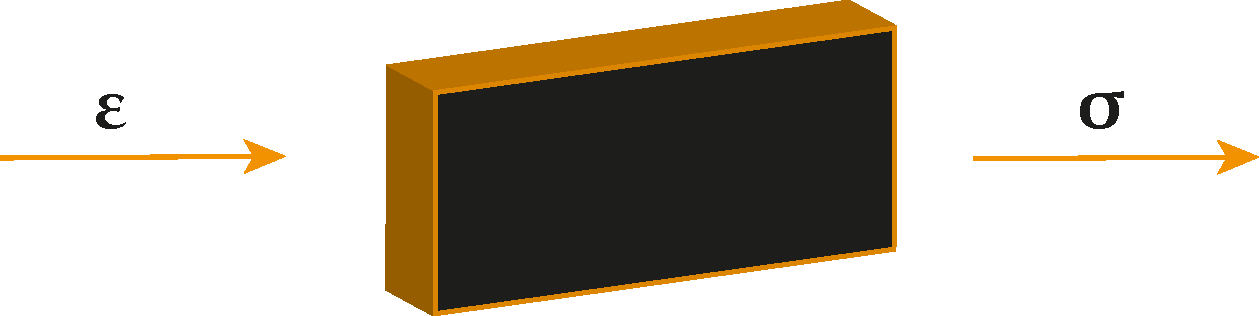
\includegraphics[width=0.8\textwidth]{Figures/surrogate/material.pdf}
  \end{minipage}
  \end{frame}

  \begin{frame}{Constitutive Modeling-FE$^2$}
  \begin{center}
    $\nabla \cdot \boldsymbol{\sigma} =0 \to  $ Equilibrium Equation 
  \end{center}
   
  \begin{minipage}{0.45\textwidth}
    \begin{block}{\color{White} Assumptions}
     \begin{itemize}
        \item Geometry 
        \item Material Model
     \end{itemize}
    \end{block} 
    \only<2> {
    \centering
      $\Downarrow$
    \begin{block}{\color{White} Parametrizations Examples}
     \begin{itemize}
        \item $V_f$, $L$
        \item $E$, $\nu$
     \end{itemize}
    \end{block}}
  \end{minipage}%
  \hspace{1cm}
  \begin{minipage}{0.45\textwidth}
    \centering
    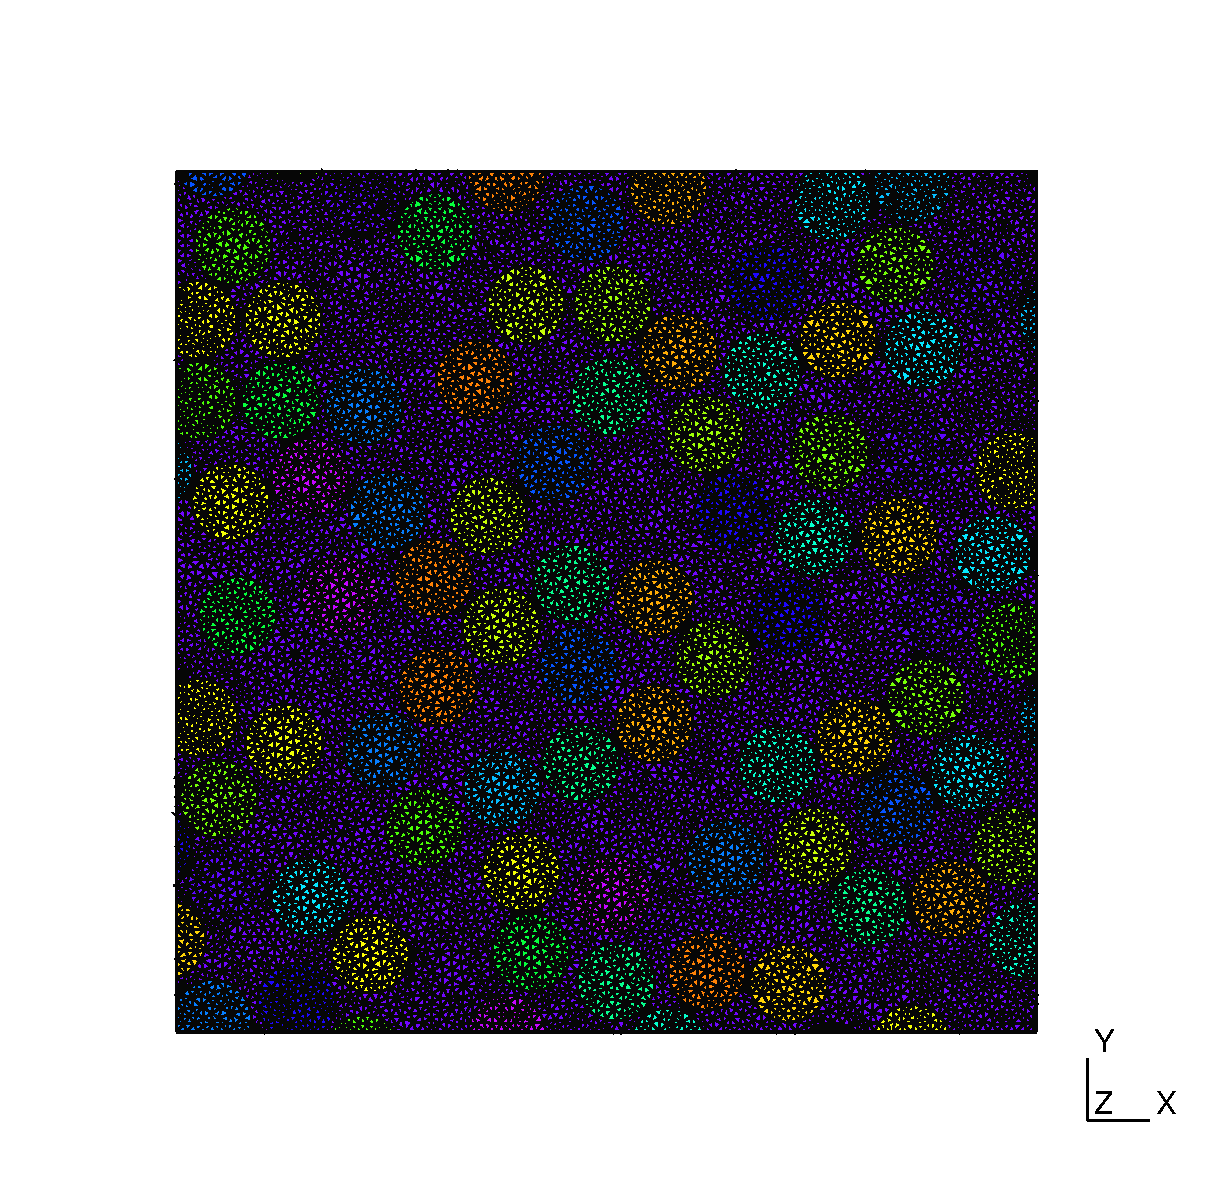
\includegraphics[width=0.9\textwidth]{Figures/surrogate/rve81.pdf}
  \end{minipage}
  \end{frame}

  \begin{frame}{Current ML Approaches}
  \centering
    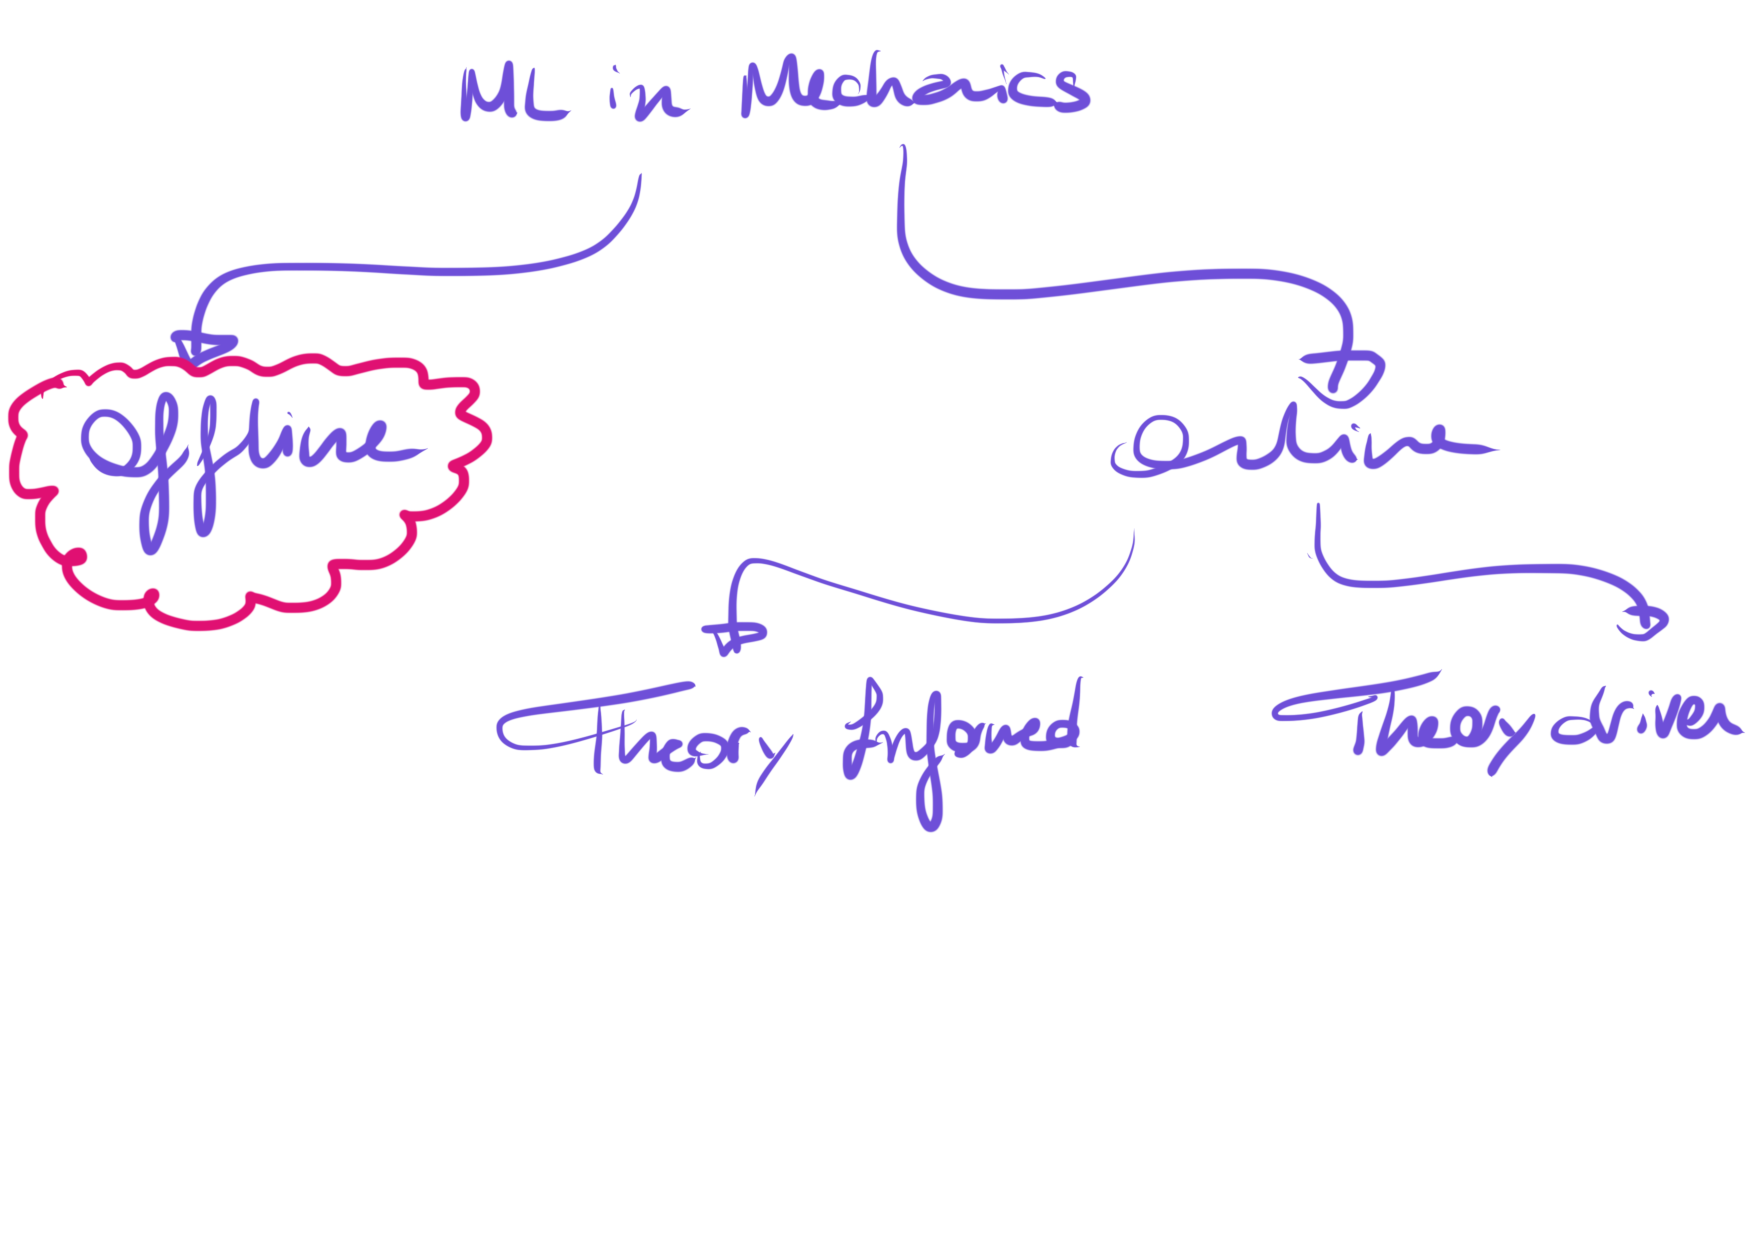
\includegraphics[width=0.8\textwidth]{Figures/surrogate/ML-Mech.pdf}
  \end{frame}

  \begin{frame}{Current ML Approaches}
  \centering
  \begin{minipage}{0.8\textwidth}
      \begin{itemize}
        \item \textit{Theory-informed}: SCA \cite{Liu2016b}, DMN \cite{Liu2019a}, etc.
        \item \textit{Theory-driven}: PINN\cite{Raissi2017}
        \item Offline: \cite{Rocha2020},\cite{Bessa2017b}
      \end{itemize}
  \end{minipage}%
  \end{frame}


\section{Observations \& Possible Paths}

\begin{frame}{Starting Point}
  \centering
    \color{Pink} Transfer Learning for DNN Applications for Constitutive Modeling \color{Black}
\begin{center}
  $\nabla \cdot \boldsymbol{\sigma} =0 \to  $ Equilibrium Equation 
\end{center}
 
\begin{minipage}{0.45\textwidth}
  \begin{block}{\color{White} Assumptions}
   \begin{itemize}
      \item Geometry 
      \item Material Model
   \end{itemize}
  \end{block} 
  \only<1> {
  \centering
    $\Downarrow$
  \begin{block}{\color{White} Parametrizations Examples}
   \begin{itemize}
      \item $V_f$, $L$
      \item $E$, $\nu$
   \end{itemize}
  \end{block}}
\end{minipage}%
\hspace{1cm}
\begin{minipage}{0.45\textwidth}
  \centering
  \begin{itemize}
      \item Learning objective: $\sigma=\mathcal{C}(\varepsilon, \cdot)$ 
  \end{itemize}
\end{minipage}
\end{frame}

\begin{frame}{Current ML-Mechanics Landscape}
\begin{minipage}{0.45\textwidth}
  \begin{block}{\color{White} Problems}<1-3>
    \begin{itemize}
      \item <3> Need of abundant data
      \item <3> Problem specific applications 
      \item <3> Single parameter considerations
    \end{itemize}
  \end{block} 
\end{minipage}%
\begin{minipage}{0.45\textwidth}
    \centering
    \color{Pink} \only<1>{Consider offline methods!} \only<2>{Why?}
  \end{minipage}
\end{frame}

\begin{frame}{Overarching Goal-A}
\centering
  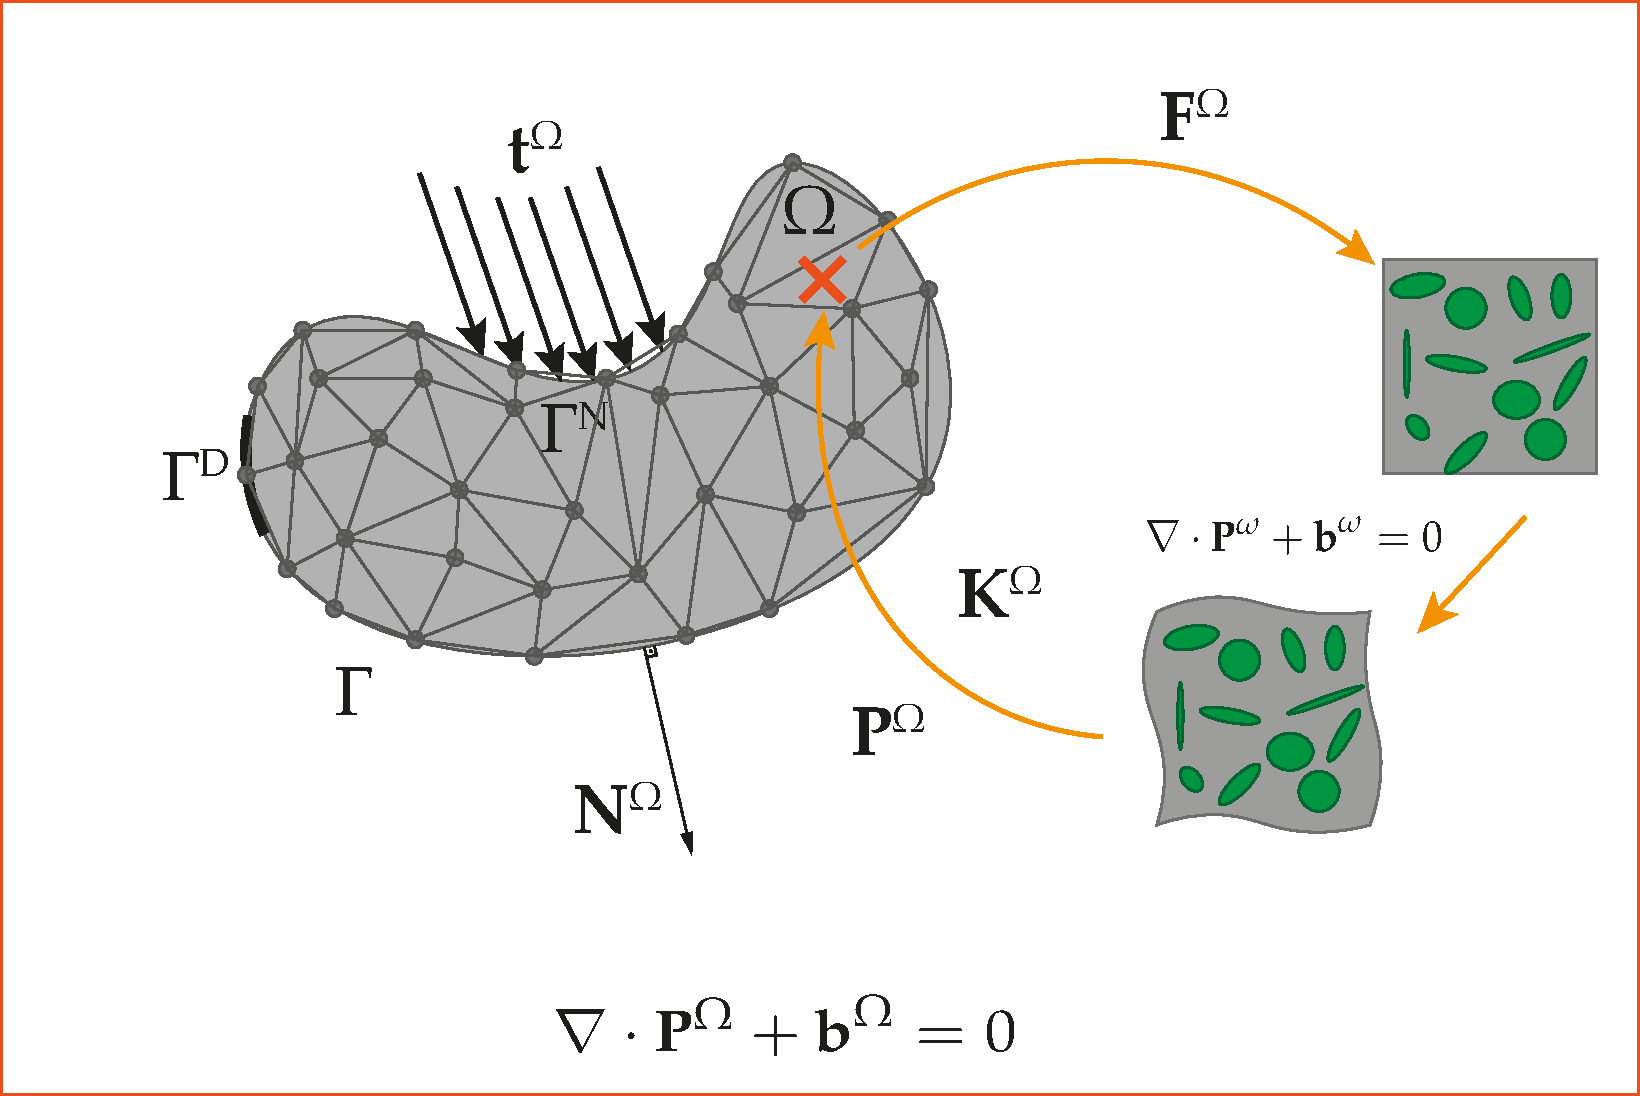
\includegraphics[width=0.45\textwidth]{Figures/myview/FE2-CONV}\hspace{1cm}\includegraphics[width=0.45\textwidth]{Figures/myview/fe2-ML}
\end{frame}

\begin{frame}{Overarching Goal-B}
\begin{minipage}{0.45\textwidth}
  \begin{block}{\color{White}Properties of $\mathcal{A}$}
  \begin{itemize}
    \item Capability to utilize past information
    \item Limited data demand 
    \item Good generalization 
  \end{itemize}
\end{block}
\end{minipage}%
  \begin{minipage}{0.5\textwidth}
    \centering
    \includegraphics[width=0.8\textwidth]{Figures/myview/fe2-ML}
  \end{minipage}
\end{frame}

\begin{frame}{Possible Paths}
  \begin{minipage}{0.6\textwidth}
    \begin{block}{\color{white}Access}
  \begin{itemize}
    \item<1> A parameterized oracle model for $\sigma=\mathcal{C}(\varepsilon, \cdot)$
  \end{itemize}
  \end{block}
  \begin{block}{\color{white}Possible Paths}
  \begin{itemize}
    \item<2> Learning the tasks space ($\sigma=\mathcal{C}(\varepsilon, \cdot))_{i=1}^M$
    \item<3> Effect of continual task observation...
    \item<4> Access to subspace of task as a whole 
    \item<5> Active sampling of tasks and data in a task
  \end{itemize}
  \end{block}
  \end{minipage}%
  \begin{minipage}{0.4\textwidth}
    \includegraphics<2-4>[width=\textwidth]{Figures/myview/tasks}
    \includegraphics<5>[width=\textwidth]{Figures/myview/task_space}
  \end{minipage}
\end{frame}

\begin{frame}{Holistic Problem}
\centering
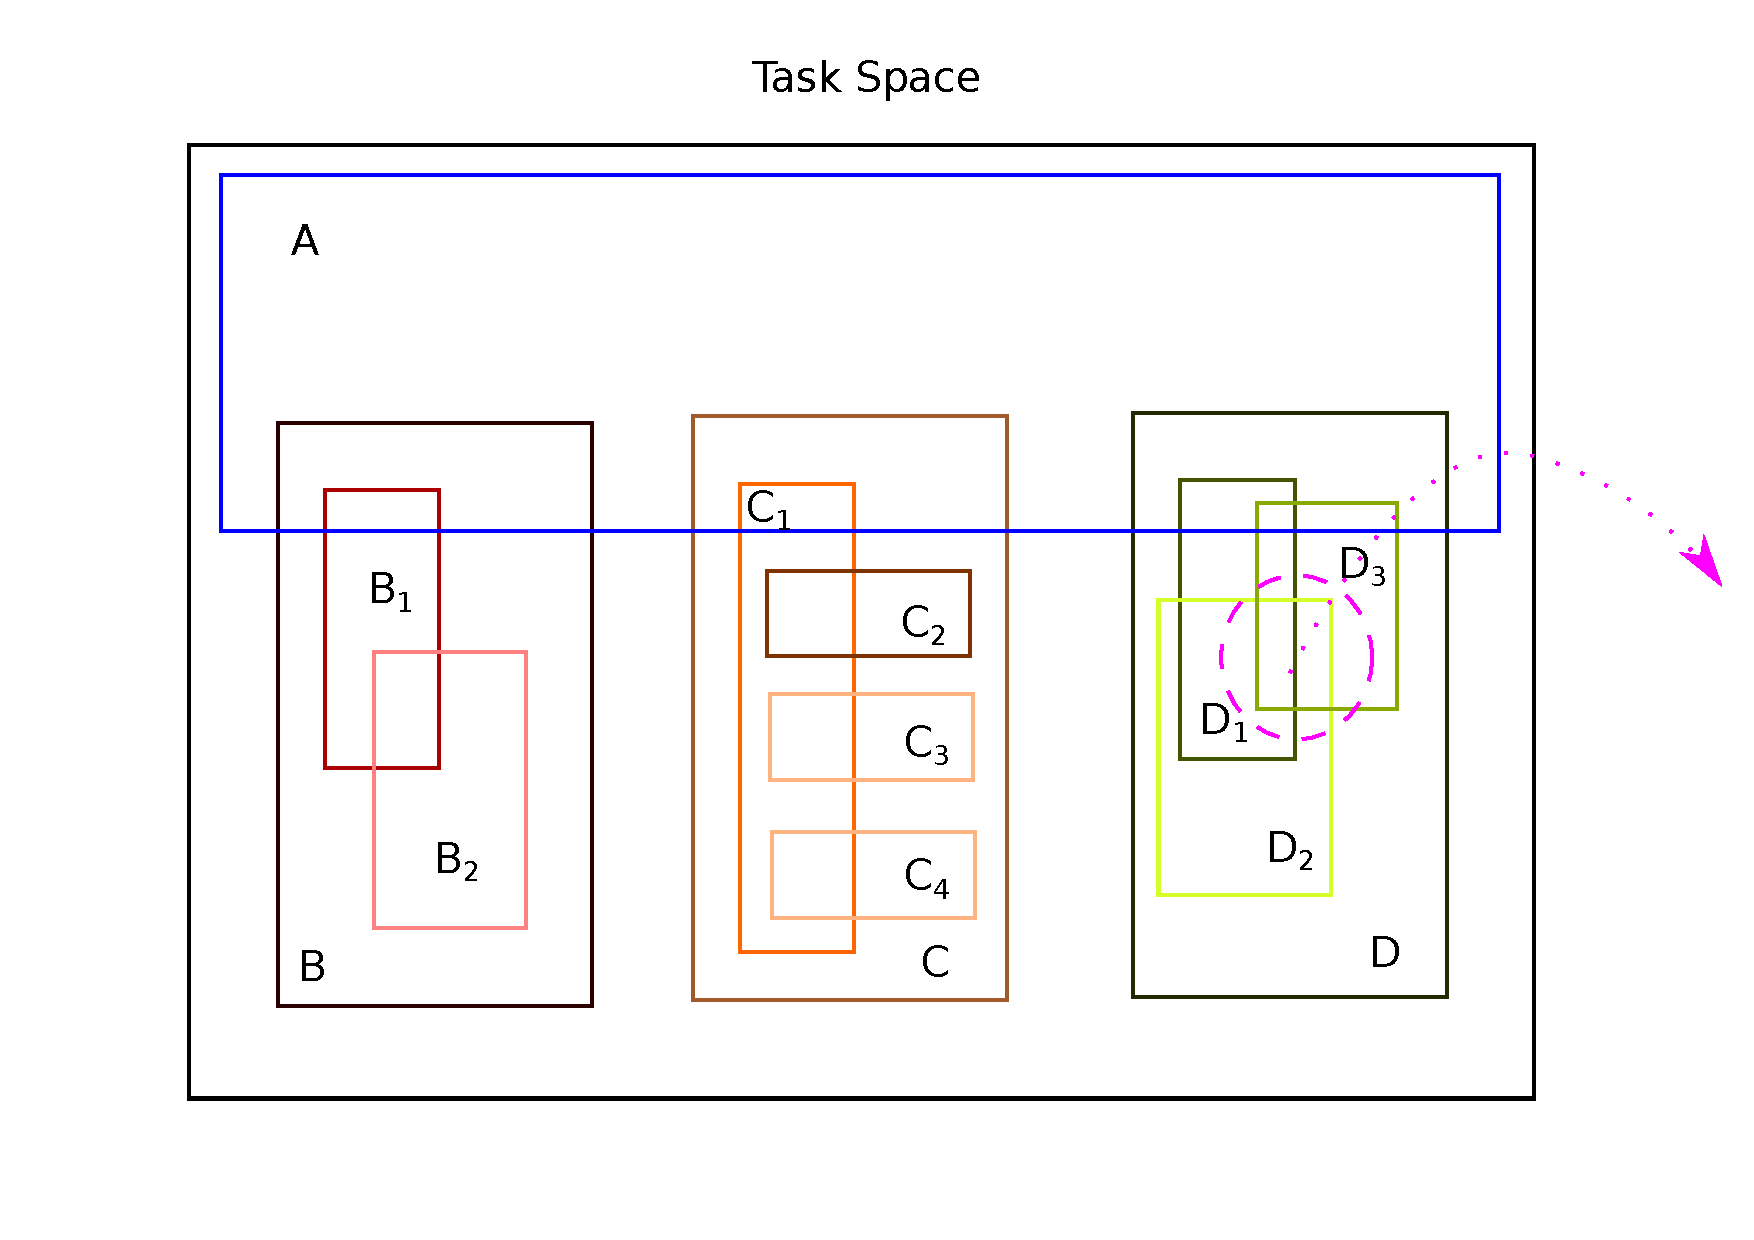
\includegraphics[width=0.6\textwidth]{Figures/myview/tasks.pdf}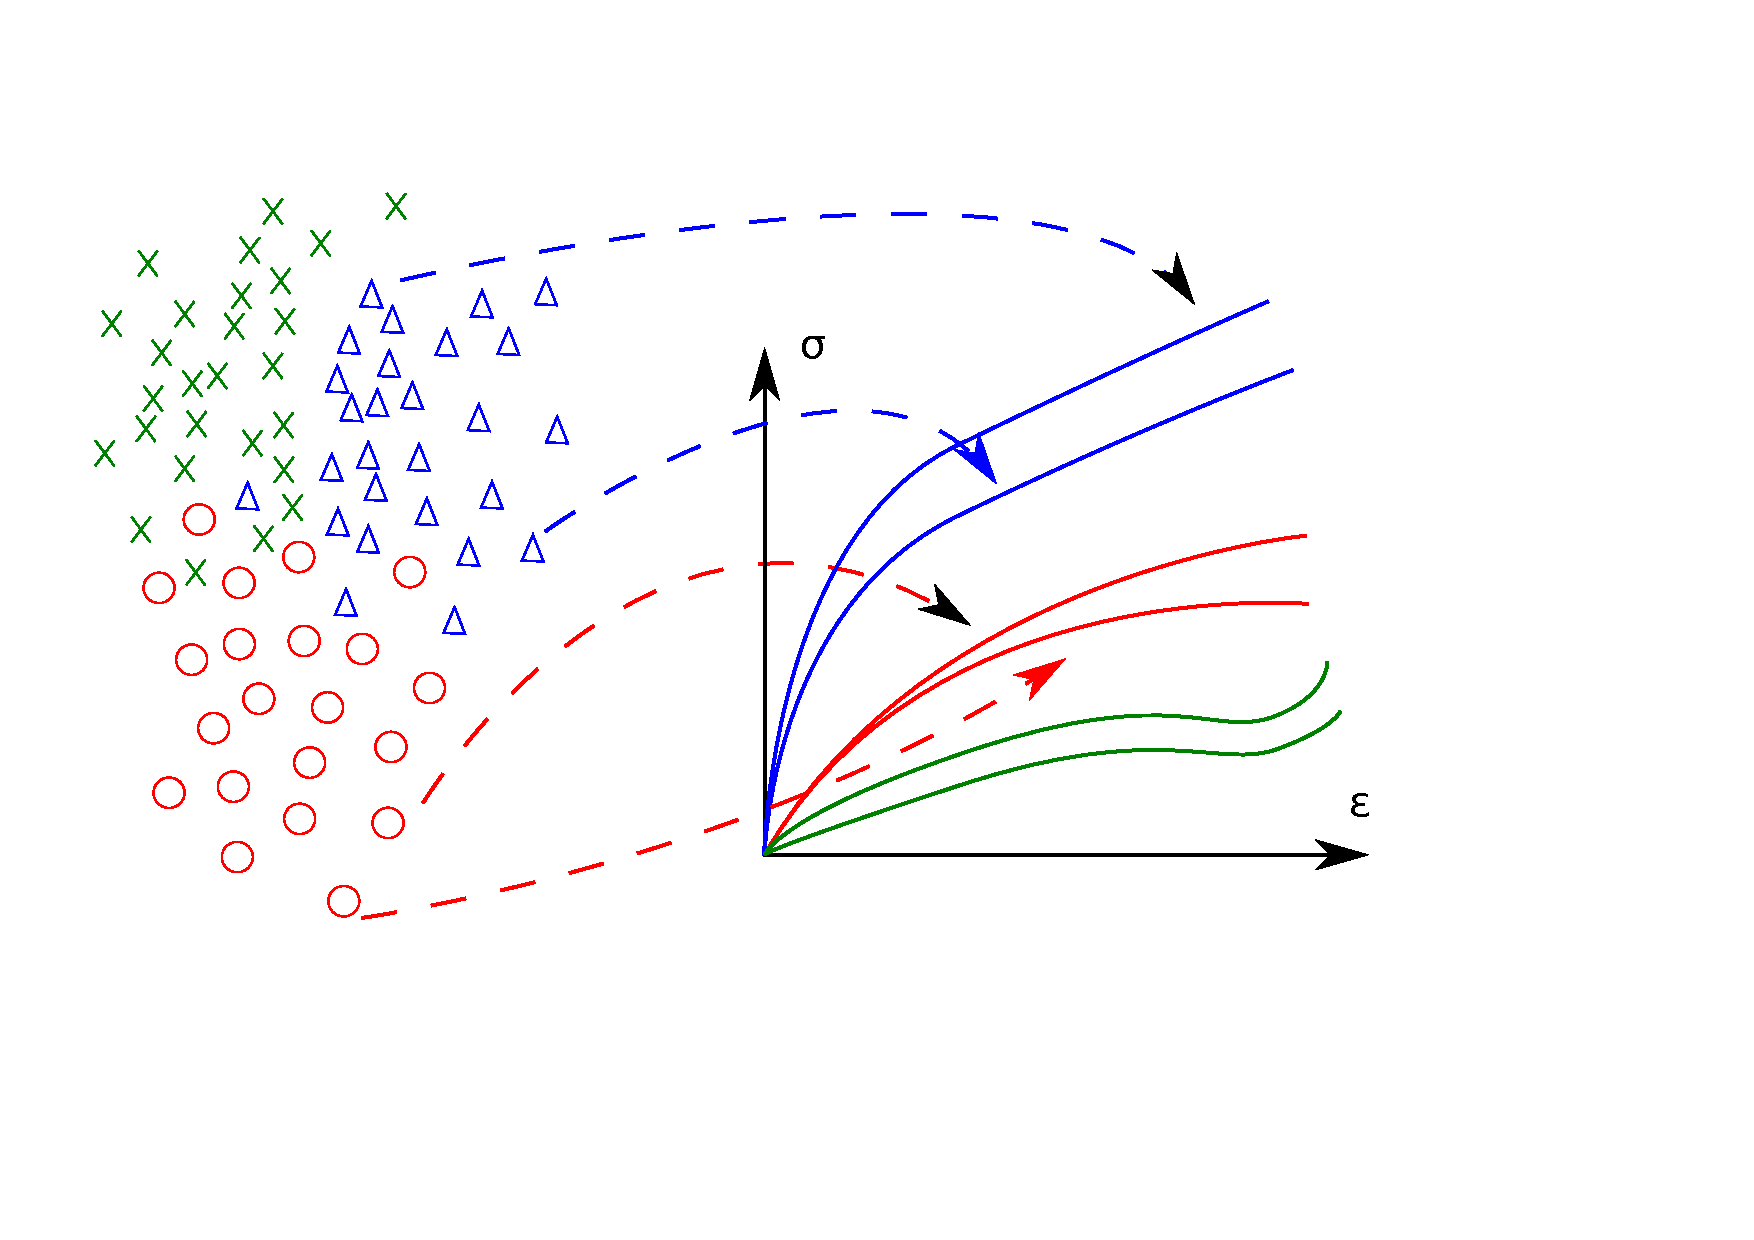
\includegraphics[width=0.4\textwidth]{Figures/myview/task_space.pdf}
\end{frame}

\begin{frame}{My work}
\centering
\begin{block}{\color{White} Until now}
  \begin{itemize}
    \item Data generation framework
  \end{itemize}
\end{block}
\begin{block}{\color{White} Currently}
  \begin{itemize}
    \item Generalization capabilities of MAML
  \end{itemize}
\end{block}
\begin{block}{\color{White} Future}
  \begin{itemize}
    \item Learning to Learn material models
    \item Domain adaptation and generalization if we consider the labels as full mappings?
  \end{itemize}
\end{block}
\end{frame}

\section{Summary}
\begin{frame}{Summary}
  \begin{itemize}
    \item Accelerate conventional PDE solution techniques (for certain problems)
    \item Learn $\sigma=\mathcal{C}(\varepsilon, \cdot)$ 
    \item Either past data or active sampling
  \end{itemize}
\end{frame}



\end{document}
